\section{Результаты}

\subsection{Выборочные коэффициенты корреляции}

\begin{table}[H]
	\begin{center}
		\begin{tabular}{|c||c|c|c|}
			\hline
			$size = 20$ & $r$ & $r_s$ & $r_q$ \\ 
			\hline 
			$E(z)$ & 0.00559 & 0.00604 & 0.00180 \\ 
			\hline 
			$E(z^2)$ & 0.05722 & 0.05508 & 0.05388 \\ 
			\hline 
			$D(z)$ & 0.05719 & 0.05504 & 0.05388 \\ 
			\hline \hline 
			$size = 60$ & $r$ & $r_s$ & $r_q$ \\ 
			\hline 
			$E(z)$ & -0.00476 & -0.00386 & -0.00260 \\ 
			\hline 
			$E(z^2)$ & 0.01807 & 0.01819 & 0.01728 \\ 
			\hline 
			$D(z)$ & 0.01805 & 0.01817 & 0.01727 \\ 
			\hline \hline 
			$size = 100$ & $r$ & $r_s$ & $r_q$ \\ 
			\hline 
			$E(z)$ & -0.00309 & -0.00270 & -0.00348 \\ 
			\hline 
			$E(z^2)$ & 0.00980 & 0.00990 & 0.01003 \\ 
			\hline 
			$D(z)$ & 0.00979 & 0.00989 & 0.01002 \\ 
			\hline
		\end{tabular}
	\end{center}
	\caption{Двумерное нормальное распределение $\rho = 0$}
\end{table} 

\begin{table}[H]
	\begin{center}
		\begin{tabular}{|c||c|c|c|}
			\hline
			$size = 20$ & $r$ & $r_s$ & $r_q$ \\ 
			\hline 
			$E(z)$ & 0.48728 & 0.46564 & 0.33940 \\ 
			\hline 
			$E(z^2)$ & 0.27003 & 0.25306 & 0.16420 \\ 
			\hline 
			$D(z)$ & 0.03259 & 0.03624 & 0.04901 \\ 
			\hline \hline 
			$size = 60$ & $r$ & $r_s$ & $r_q$ \\ 
			\hline 
			$E(z)$ & 0.49830 & 0.47663 & 0.33273 \\ 
			\hline 
			$E(z^2)$ & 0.25762 & 0.23768 & 0.12535 \\ 
			\hline 
			$D(z)$ & 0.00932 & 0.01050 & 0.01464 \\ 
			\hline \hline 
			$size = 100$ & $r$ & $r_s$ & $r_q$ \\ 
			\hline 
			$E(z)$ & 0.49535 & 0.47482 & 0.32672 \\ 
			\hline 
			$E(z^2)$ & 0.25123 & 0.23225 & 0.11668 \\ 
			\hline 
			$D(z)$ & 0.00586 & 0.00679 & 0.00993 \\ 
			\hline 
		\end{tabular}
	\end{center}
	\caption{Двумерное нормальное распределение $\rho = 0.5$}
\end{table} 

\begin{table}[H]
	\begin{center}
		\begin{tabular}{|c||c|c|c|}
		\hline
		$size = 20$ & $r$ & $r_s$ & $r_q$ \\ 
		\hline 
		$E(z)$ & 0.89710 & 0.86851 & 0.69720 \\ 
		\hline 
		$E(z^2)$ & 0.80705 & 0.75889 & 0.51384 \\ 
		\hline 
		$D(z)$ & 0.00225 & 0.00458 & 0.02775 \\ 
		\hline \hline 
		$size = 60$ & $r$ & $r_s$ & $r_q$ \\ 
		\hline 
		$E(z)$ & 0.89786 & 0.88201 & 0.70300 \\ 
		\hline 
		$E(z^2)$ & 0.80679 & 0.77903 & 0.50279 \\ 
		\hline 
		$D(z)$ & 0.00064 & 0.00110 & 0.00858 \\ 
		\hline \hline 
		$size = 100$ & $r$ & $r_s$ & $r_q$ \\ 
		\hline 
		$E(z)$ & 0.89863 & 0.88605 & 0.70752 \\ 
		\hline 
		$E(z^2)$ & 0.80794 & 0.78571 & 0.50582 \\ 
		\hline 
		$D(z)$ & 0.00039 & 0.00062 & 0.00524 \\ 
		\hline 
		\end{tabular}
	\end{center}
	\caption{Двумерное нормальное распределение $\rho = 0.9$}
\end{table} 

\begin{table}[H]
	\begin{center}
		\begin{tabular}{|c||c|c|c|}
			\hline
			$size = 20$ & $r$ & $r_s$ & $r_q$ \\ 
			\hline 
			$E(z)$ & 0.78243 & 0.74746 & 0.56700 \\ 
			\hline 
			$E(z^2)$ & 0.62071 & 0.57078 & 0.35628 \\ 
			\hline 
			$D(z)$ & 0.00851 & 0.01208 & 0.03479 \\ 
			\hline \hline 
			$size = 60$ & $r$ & $r_s$ & $r_q$ \\ 
			\hline 
			$E(z)$ & 0.79042 & 0.77002 & 0.58047 \\ 
			\hline 
			$E(z^2)$ & 0.62747 & 0.59652 & 0.34752 \\ 
			\hline 
			$D(z)$ & 0.00271 & 0.00359 & 0.01058 \\ 
			\hline \hline 
			$size = 100$ & $r$ & $r_s$ & $r_q$ \\ 
			\hline 
			$E(z)$ & 0.78787 & 0.76874 & 0.57448 \\ 
			\hline 
			$E(z^2)$ & 0.62225 & 0.59306 & 0.33664 \\ 
			\hline 
			$D(z)$ & 0.00151 & 0.00210 & 0.00662 \\ 
			\hline 
		\end{tabular}
	\end{center}
	\caption{Смесь нормальных распределений}
\end{table} 

\subsection{Эллипсы рассеивания}

Для уравнения эллипса выбиралиссь $\sigma_x = 1$, $\sigma_y = 1$

\begin{figure}[H]
	\begin{tabular}{cccc}
		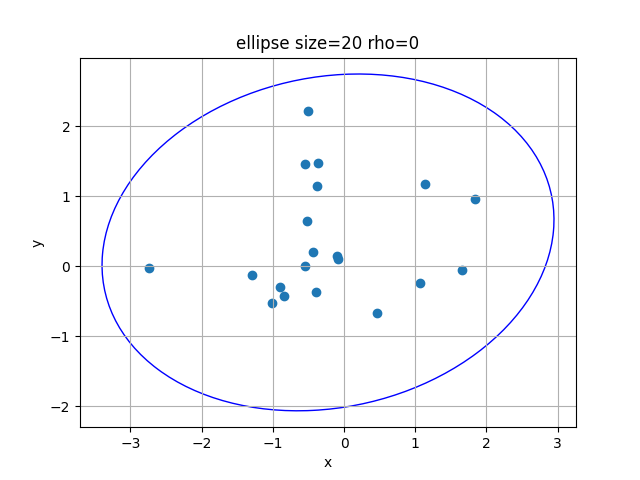
\includegraphics[scale=0.3]{ellipse_20_0.png}
		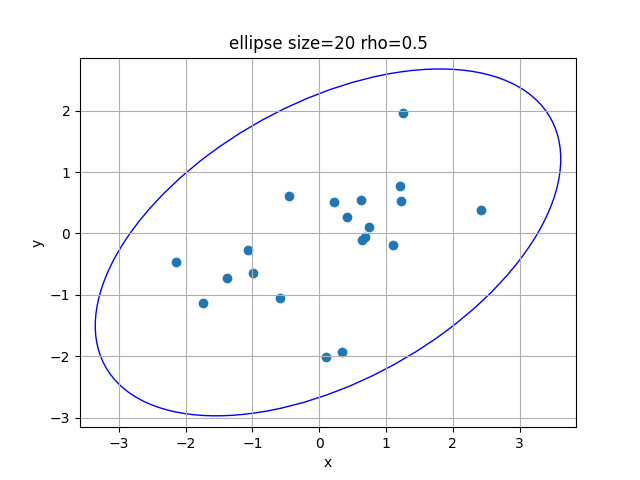
\includegraphics[scale=0.3]{ellipse_20_0.5.png}
		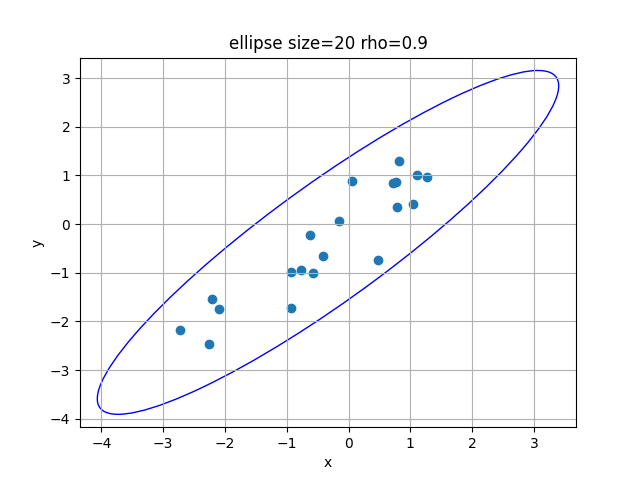
\includegraphics[scale=0.3]{ellipse_20_0.9.png}
		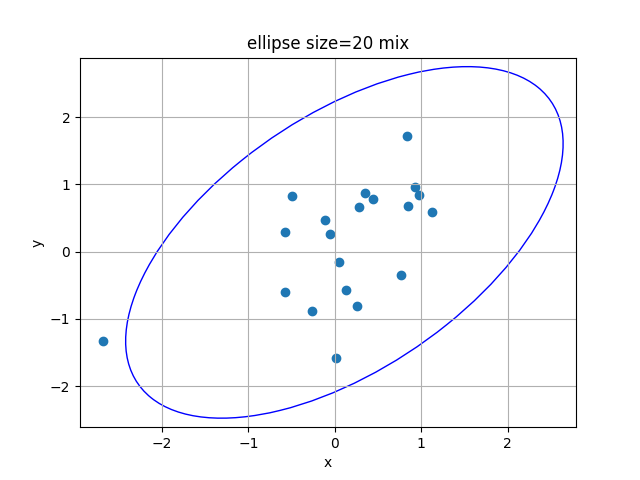
\includegraphics[scale=0.3]{ellipse_20_mix.png}
	\end{tabular}
	\caption{Эллипсы рассеивания для двумерного нормального распределения и смеси нормальных распределений, n = 20}
\end{figure}

\begin{figure}[H]
	\begin{tabular}{cccc}
		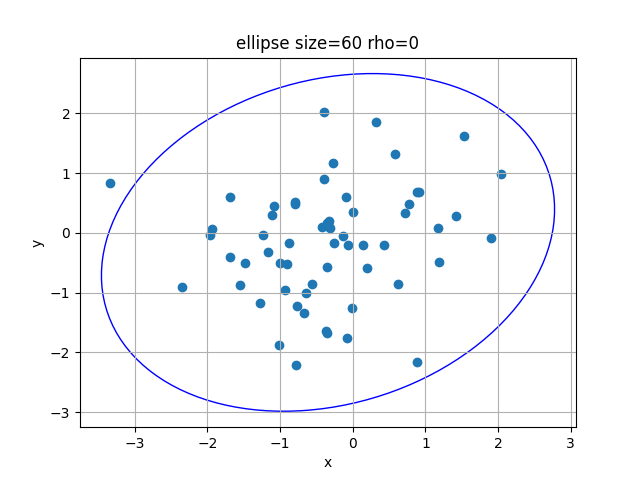
\includegraphics[scale=0.3]{ellipse_60_0.png}
		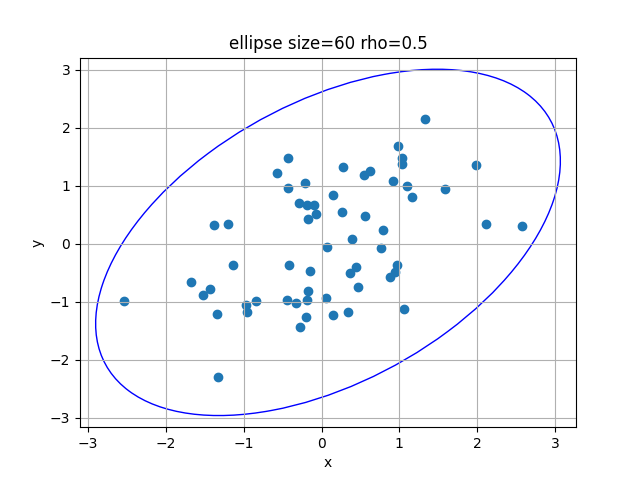
\includegraphics[scale=0.3]{ellipse_60_0.5.png}
		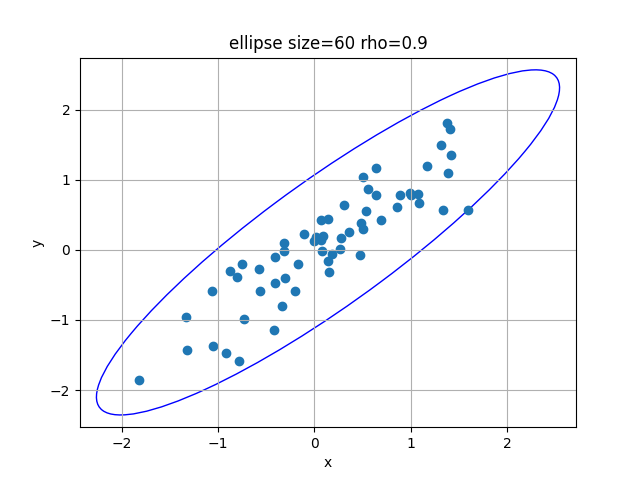
\includegraphics[scale=0.3]{ellipse_60_0.9.png}
		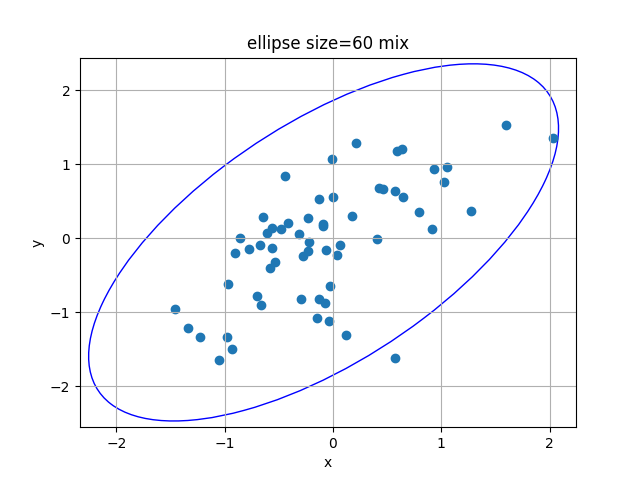
\includegraphics[scale=0.3]{ellipse_60_mix.png}
	\end{tabular}
	\caption{Эллипсы рассеивания для двумерного нормального распределения и смеси нормальных распределений, n = 60}
\end{figure}

\begin{figure}[H]
	\begin{tabular}{cccc}
		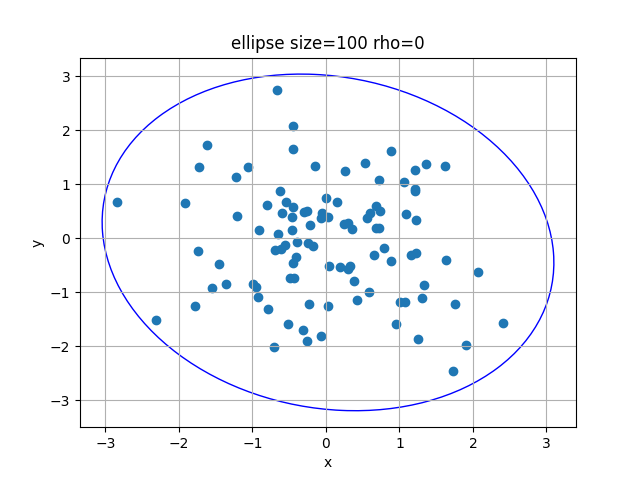
\includegraphics[scale=0.3]{ellipse_100_0.png}
		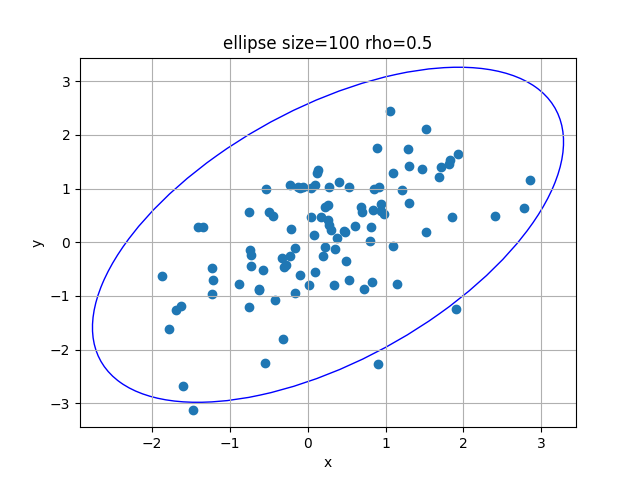
\includegraphics[scale=0.3]{ellipse_100_0.5.png}
		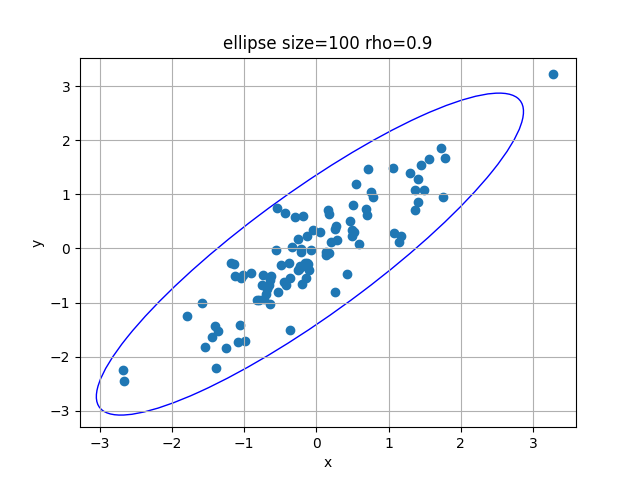
\includegraphics[scale=0.3]{ellipse_100_0.9.png}
		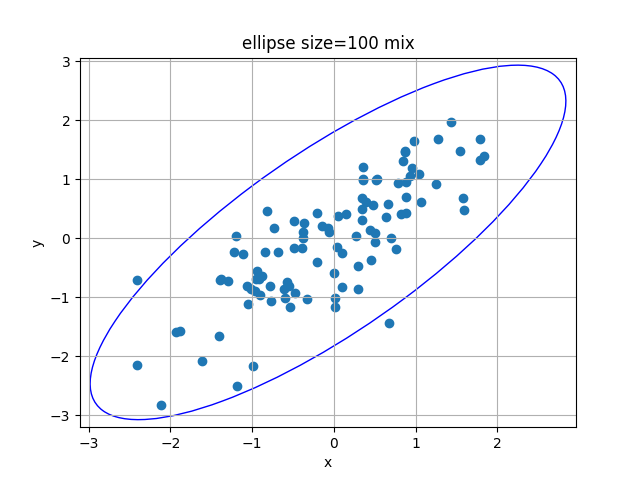
\includegraphics[scale=0.3]{ellipse_100_mix.png}
	\end{tabular}
	\caption{Эллипсы рассеивания для двумерного нормального распределения и смеси нормальных распределений, n = 100}
\end{figure}

\subsection{Оценки коэффициентов линейной регрессии}

Метрика удаленности: $distance = \sum\limits_{i=0}^{n} (y_{model}[i] - y_{regr}[i])^{2} $

\subsubsection{Выборка без возмущений}

Критерий наименьших квадратов: $\hat{a} \approx 2.33932, \quad \hat{b} \approx 2.03879$ \\

Критерий наименьших модулей: $\hat{a} \approx 2.07868, \quad \hat{b} \approx 2.02210$

\begin{figure}[H]
	\begin{center}
		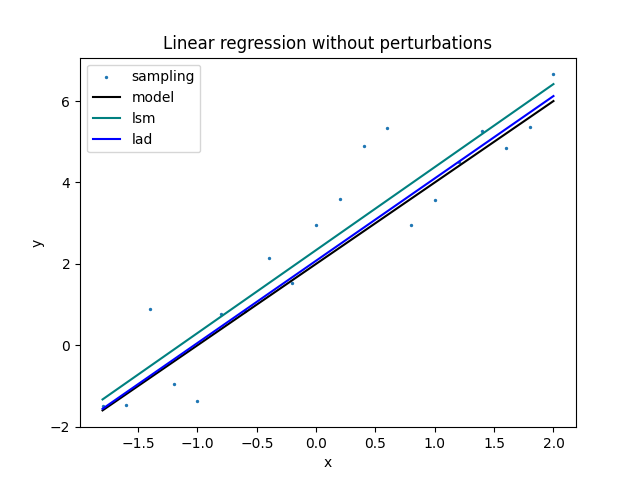
\includegraphics[scale=0.7]{regression_without_pert.png}
	\end{center}
	\caption{Линейная регрессия для выборки без возмущений}
\end{figure}

\subsubsection{Выборка с возмущениями}

Были внесены возмущения 10 и -10 в $y_1$ и $y_{20}$ соответственно. \\

Критерий наименьших квадратов: $\hat{a} \approx 2.48218, \quad \hat{b} \approx 0.61022$ \\

Критерий наименьших модулей: $\hat{a} \approx 2.17987, \quad \hat{b} \approx 1.77162$

\begin{figure}[H]
	\begin{center}
		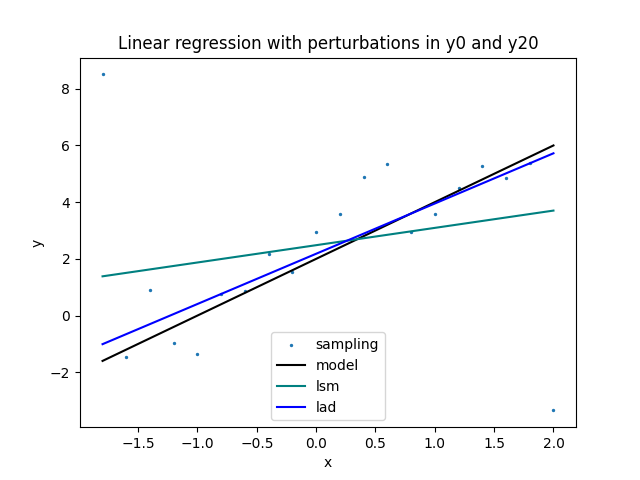
\includegraphics[scale=0.7]{regression_with_pert.png}
	\end{center}
	\caption{Линейная регрессия для выборки с возмущениями}
\end{figure}

\subsection{Оценки максимального правдоподобия}

Оценки для выборки размером 100 элементов стандартного нормального распредления, полученные методом максимального правдоподобия: \\
$\hat{\mu} = 0.04, \hat{\sigma} = 0.93 $

\subsection{Проверка гипотезы о законе распределения генеральной совокупности методом $\chi^2$ }

\subsubsection{Нормальное распределение, n=100}

$\alpha = 0.05$ \\
$\chi^{2}_{0.95}(7) \approx 14.07$ \\

\begin{table}[H]
	\begin{center}
		\begin{tabular}{|c|c|c|c|c|c|c|}
			\hline
			$i$ & limits & $n_i$ & $p_i$ & $np_i$ & $n_i - np_i$ & $\dfrac{(n_i-np_i)^2}{np_i}$ \\
			\hline
			1 & [$-\infty$, -1.1] & 13.0 & 0.1357 & 13.57 & -0.57 & 0.02 \\
			2 & [-1.1, -0.73] & 4.0 & 0.096 & 9.6 & -5.6 & 3.27 \\
			3 & [-0.73, -0.37] & 10.0 & 0.1253 & 12.53 & -2.53 & 0.51 \\
			4 & [-0.37, 0.0] & 17.0 & 0.1431 & 14.31 & 2.69 & 0.51 \\
			5 & [0.0, 0.37] & 21.0 & 0.1431 & 14.31 & 6.69 & 3.13 \\
			6 & [0.37, 0.73] & 10.0 & 0.1253 & 12.53 & -2.53 & 0.51 \\
			7 & [0.73, 1.1] & 13.0 & 0.096 & 9.6 & 3.4 & 1.2 \\
			8 & [1.1, $\infty$] & 12.0 & 0.1357 & 13.57 & -1.57 & 0.18 \\
			\hline
			$\sum$ & - & 100.0 & 1.0 & 100.0 & 0.0 & 9.33\\
			\hline
		\end{tabular}
	\end{center}
	\caption{Вычисление $\chi_{B}^2$ при проверке гипотезы $H_0$ для выборки нормального распределения, n=100}
\end{table} 

$\chi_{B}^2 = 9.33$, следовательно  $\chi_{B}^2 <\chi^{2}_{0.95}(7)$ \\

\subsubsection{Распределение Лапласа, n=20}

$\alpha = 0.05$ \\
$\chi^{2}_{0.95}(4) \approx 9.49$ \\

\begin{table}[H]
	\begin{center}
		\begin{tabular}{|c|c|c|c|c|c|c|}
			\hline
			$i$ & limits & $n_i$ & $p_i$ & $np_i$ & $n_i - np_i$ & $\dfrac{(n_i-np_i)^2}{np_i}$ \\
			\hline
			1 & [$-\infty$, -1.1] & 0.0 & 0.1357 & 2.71 & -2.71 & 2.71 \\
			2 & [-1.1, -0.37] & 6.0 & 0.2213 & 4.43 & 1.57 & 0.56 \\
			3 & [-0.37, 0.37] & 9.0 & 0.2861 & 5.72 & 3.28 & 1.88 \\
			4 & [0.37, 1.1] & 4.0 & 0.2213 & 4.43 & -0.43 & 0.04 \\
			5 & [1.1, $\infty$] & 1.0 & 0.1357 & 2.71 & -1.71 & 1.08 \\
			\hline
			$\sum$ & - & 20.0 & 1.0 & 20.0 & 0.0 & 6.27\\
			\hline
		\end{tabular}
	\end{center}
	\caption{Вычисление $\chi_{B}^2$ при проверке гипотезы $H_0$ для выборки распределения Лапласа, n=20}
\end{table}

$\chi_{B}^2 = 6.27$, следовательно  $\chi_{B}^2 <\chi^{2}_{0.95}(7)$ \\
\subsubsection{Равномерное распределение, n=20}

$\alpha = 0.05$ \\
$\chi^{2}_{0.95}(4) \approx 9.49$ \\

\begin{table}[H]
	\begin{center}
		\begin{tabular}{|c|c|c|c|c|c|c|}
			\hline
			$i$ & limits & $n_i$ & $p_i$ & $np_i$ & $n_i - np_i$ & $\dfrac{(n_i-np_i)^2}{np_i}$ \\
			\hline
			1 & [$-\infty$, -1.1] & 4.0 & 0.1357 & 2.71 & 1.29 & 0.61 \\
			2 & [-1.1, -0.37] & 5.0 & 0.2213 & 4.43 & 0.57 & 0.07 \\
			3 & [-0.37, 0.37] & 2.0 & 0.2861 & 5.72 & -3.72 & 2.42 \\
			4 & [0.37, 1.1] & 4.0 & 0.2213 & 4.43 & -0.43 & 0.04 \\
			5 & [1.1, $\infty$] & 5.0 & 0.1357 & 2.71 & 2.29 & 1.93 \\
			\hline
			$\sum$ & - & 20.0 & 1.0 & 20.0 & 0.0 & 5.07\\
			\hline
		\end{tabular}
	\end{center}
	\caption{Вычисление $\chi_{B}^2$ при проверке гипотезы $H_0$ для выборки равномерного распределения, n=20}
\end{table} 

$\chi_{B}^2 = 5.07$, следовательно  $\chi_{B}^2 <\chi^{2}_{0.95}(7)$ \\

\subsection{Доверительные интервалы для параметров нормального распределения}

\begin{figure}[H]
	\begin{tabular}{cccc}
		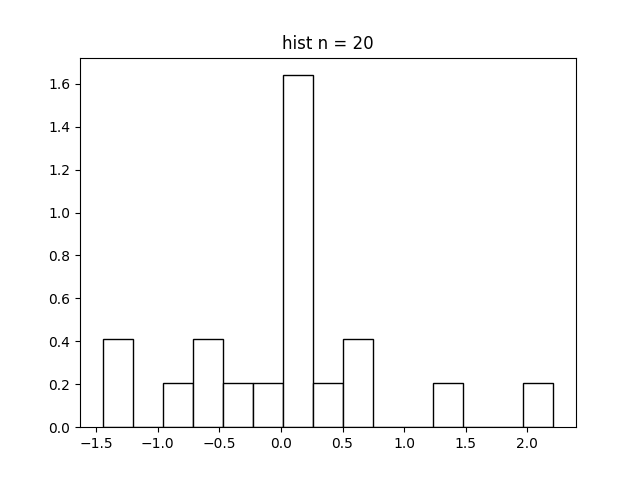
\includegraphics[scale=0.3]{hist_n_20.png}
		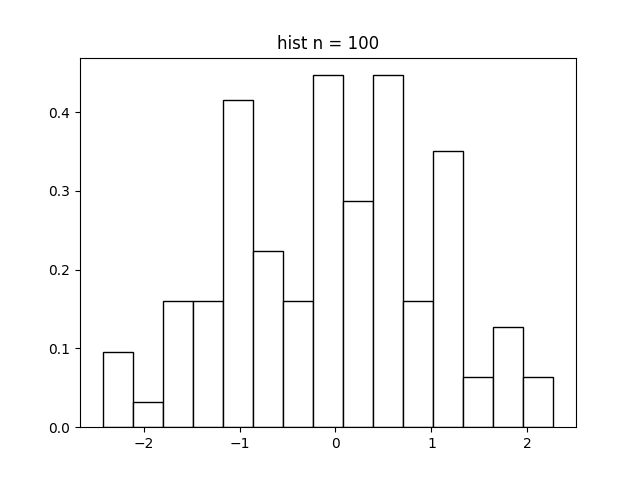
\includegraphics[scale=0.3]{hist_n_100.png}
		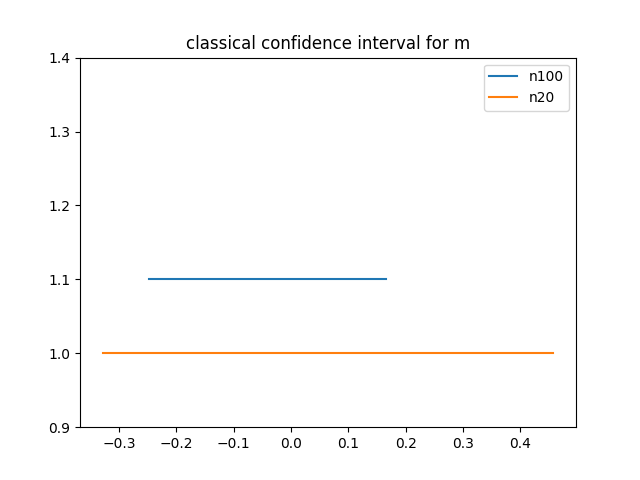
\includegraphics[scale=0.3]{classic_m.png}
		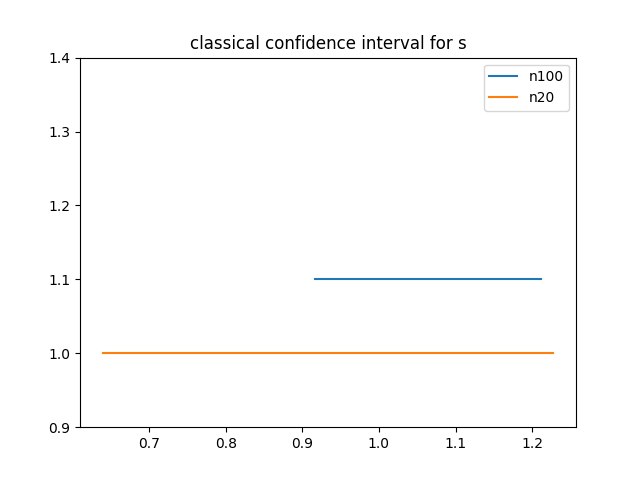
\includegraphics[scale=0.3]{classic_s.png}
	\end{tabular}
	\caption{Гистограммы нормальных распределений и доверительные интервалы их параметров}
\end{figure}

\begin{table}[H]
	\begin{center}
		\begin{tabular}{|c|c|c|}
			\hline 
			n & $m$ & $\sigma$ \\
			\hline \hline 
			20 & [-0.33, 0.46] & [0.64, 1.23] \\
			\hline 
			100 & [-0.25, 0.17] & [0.92, 1.21] \\
			\hline
		\end{tabular}
	\end{center}
	\caption{Доверительные интервалы для параметров нормального распределения}
\end{table} 

\subsection{Доверительные интервалы для параметров произвольного распределения. Ассимптотический подход}


\begin{figure}[H]
	\begin{tabular}{cccc}
		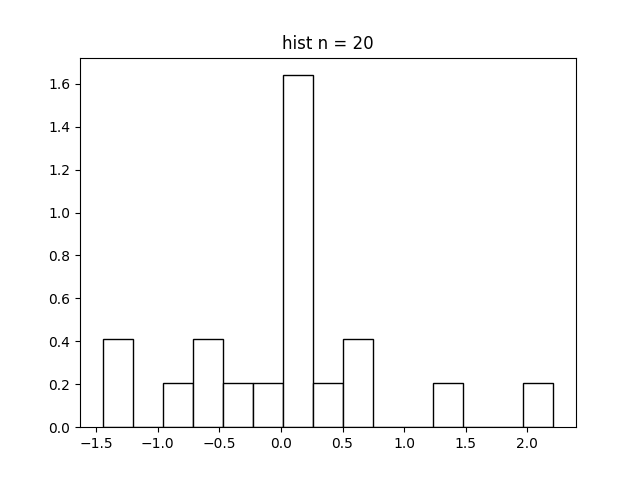
\includegraphics[scale=0.3]{hist_n_20.png}
		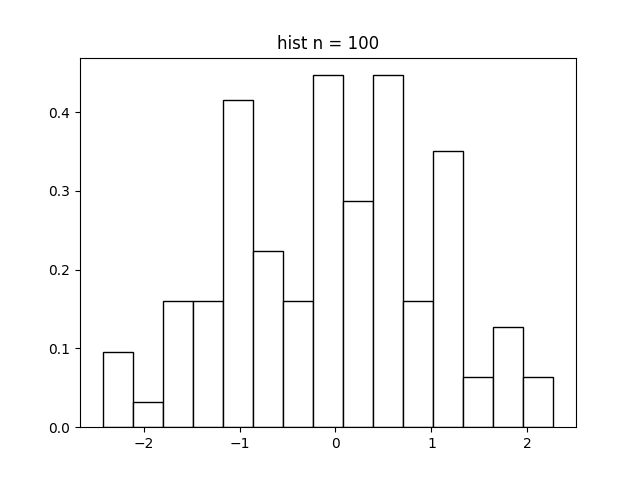
\includegraphics[scale=0.3]{hist_n_100.png}
		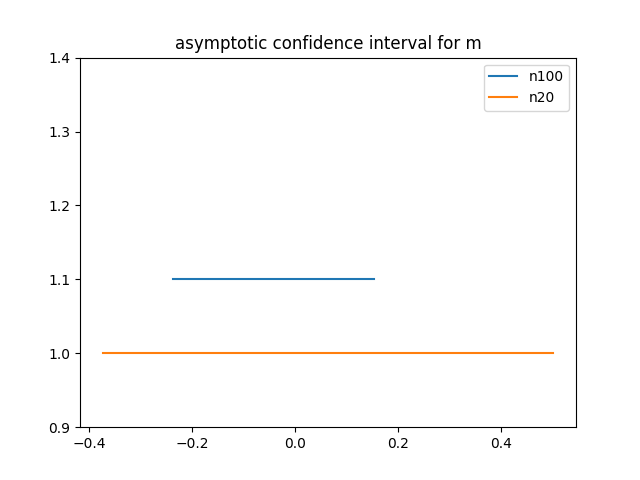
\includegraphics[scale=0.3]{asymptotic_m.png}
		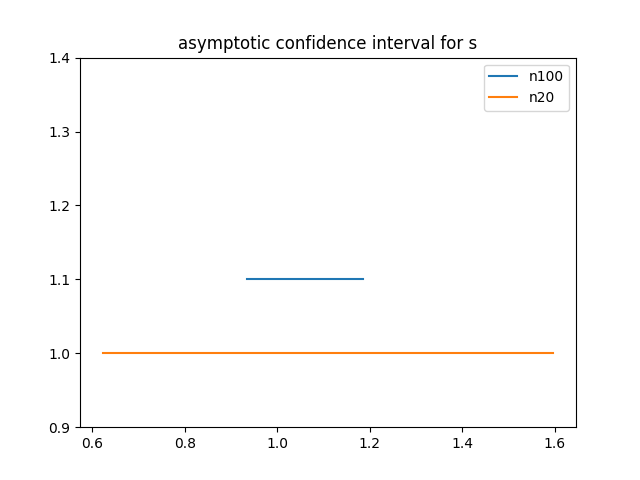
\includegraphics[scale=0.3]{asymptotic_s.png}
	\end{tabular}
	\caption{Гистограммы нормальных распределений и доверительные интервалы их параметров. Ассимптотический подход}
\end{figure}

\begin{table}[H]
	\begin{center}
		\begin{tabular}{|c|c|c|}
			\hline 
			n & $m$ & $\sigma$ \\
			\hline \hline 
			20 & [-0.37, 0.50] & [0.62, 1.60] \\
			\hline 
			100 & [-0.24, 0.15] & [0.94, 1.19] \\
			\hline
		\end{tabular}
	\end{center}
	\caption{Доверительные интервалы для параметров произвольного распределения. Ассимптотический подход}
\end{table} 

